\documentclass[UTF8,a4paper]{ctexart}

% ==========Preamble==========
\usepackage{graphicx}
\usepackage{listings}
\usepackage{apacite}
\usepackage{url}
\usepackage{fancyhdr}
\usepackage{geometry}
\usepackage[font=small,labelfont=bf,labelsep=quad,format=hang,textfont=it]{caption}
\usepackage{booktabs}
\usepackage{graphicx}
\usepackage{float}
\usepackage{xcolor}

\definecolor{commentcolor}{RGB}{85,139,78}
\definecolor{stringcolor}{RGB}{206,145,108}
\definecolor{keywordcolor}{RGB}{34,34,250}
\definecolor{backcolor}{RGB}{220,220,220}

\pagestyle{plain}
\CTEXsetup[format=\Large\bfseries]{section}
\bibliographystyle{apacite}
\DeclareGraphicsExtensions{.eps,.pdf,.jpg,.png}

%设置代码
\lstset{
	%backgroundcolor=\color{red!50!green!50!blue!50},%代码块背景色为浅灰色
%	rulesepcolor= \color{gray}, %代码块边框颜色
    commentstyle=\color{commentcolor},	%注释颜色
	keywordstyle=\color{keywordcolor},	%关键词颜色
	stringstyle=\color{stringcolor},	%字符串颜色
	breaklines=true,  %代码过长则换行
	numbers=left, %行号在左侧显示
	numberstyle= \small,%行号字体
	%keywordstyle= \color{blue},%关键字颜色
	commentstyle=\color{gray}, %注释颜色
%	frame=shadowbox%用方框框住代码块
	frame=single,
	escapeinside=``    % 代码包含中文
}

% 设置图表搜索路径, 可以给图表文件夹取如下名字
\graphicspath{{img/}}

% ==========Title==========

\title{\bfseries 第二章作业 } 
\author{\bfseries 谈昊\quad2020E8013282037}

% Your name in the first blank and your additional information in \thanks{}
\date{}
% delete \today if you don't want the date

% ==========Document==========

\begin{document}
\maketitle



\paragraph{Question}
\begin{itemize}
    \item 设以下模式类别具有正态概率密度函数:
    \begin{itemize}
        \item $\omega _1 :{(0,0)^T, (2 ,0)^T, (2 ,2)^T, (0 ,2)^T}$
        \item $\omega _2:{(4 ,4)^T, (6 ,4)^T, (6 ,6)^T, (4 ,6)^T}$
    \end{itemize}

    \begin{itemize}
        \item[(1)] 设$P(\omega _1)= P(\omega _2)=1/2$,求这两类模式之间的贝叶斯判别界面的方程式。
        \item[(2)] 绘出判别界面。
    \end{itemize}
    \item 编写两类正态分布模式的贝叶斯分类程序。(可选例题或上述作业题为分类模式)

\end{itemize}

\paragraph{Answer}
\begin{itemize}
    \item 判别方程式为:$-4.0*x_1-4.0*x_2+24.0 = 0$
    \item 判别界面:
    \begin{figure}[H]
    \centering
    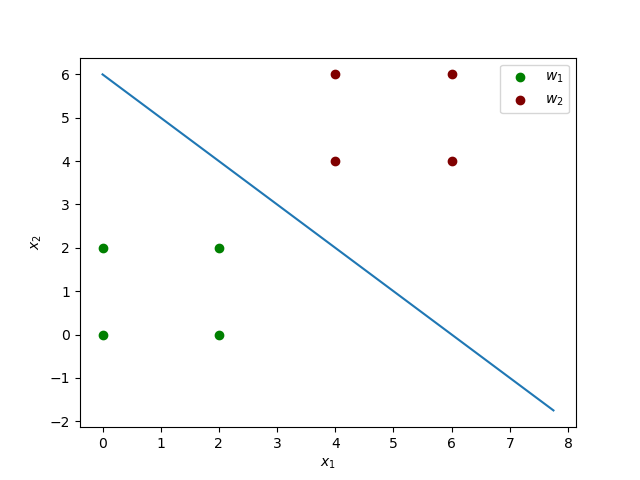
\includegraphics[width = 0.65\textwidth]{myplot.png}
    
    \label{fig:007}
    \end{figure}
    \item 代码如下:

        \begin{lstlisting}[language={Python}]
            import numpy as np


            class byers():
                def __init__(self):
                    self.w_1 = np.array([[0, 0], [2, 0], [2, 2], [0, 2]])
                    self.w_2 = np.array([[4, 4], [6, 4], [6, 6], [4, 6]])
                    self.mean_1 = self._get_mean(self.w_1)
                    self.mean_2 = self._get_mean(self.w_2)
                    self.cov = self._get_cov(self.w_1, self.mean_1)
            
                    self.w, self.b = self._get_line()
                    self._plot()
            
                def _get_mean(self, x):
                    return np.mean(x, axis=0)
            
                def _get_cov(self, x, m):
                    return np.matmul((x - m).T, x - m) / x.shape[0]
            
                def _matmul(self, x, y, z):
                    return np.matmul(np.matmul(x, y), z)
            
                def _get_line(self):
                    cov_ = np.linalg.inv(self.cov)
                    b = 0.5 * (self._matmul(self.mean_2.T, cov_, self.mean_2) - self._matmul(self.mean_1.T, cov_, self.mean_1))
                    w = np.matmul((self.mean_1 - self.mean_2).T, cov_)
                    line = ''
                    for i, item in enumerate(w.data):
                        flag = '+' if item > 0 else ''
                        line += flag + str(item) + '*x_' + str(i + 1)
                    flag = '+' if b > 0 else ''
                    line += flag + str(b)
                    print(line)
                    return w, b
            
                def _plot(self):
                    import matplotlib.pyplot as plt
                    x_1 = [x[0] for x in self.w_1.data.obj]
                    y_1 = [x[1] for x in self.w_1.data.obj]
            
                    x_2 = [x[0] for x in self.w_2.data.obj]
                    y_2 = [x[1] for x in self.w_2.data.obj]
            
                    fig = plt.figure()
            

                    X = np.arange(0, 8, 0.25)
            
                    a1 = self.w.data[0]
                    a2 = self.w.data[1]
                    Y = (-a1 * X - self.b) / a2
            

                    plt.plot(X, Y)
                    plt.xlabel(r"$x_1$")
                    plt.ylabel(r"$x_2$")
                    plt.scatter(x_1, y_1, label=r'$w_1$', color=(0., 0.5, 0.))
                    plt.scatter(x_2, y_2, label=r'$w_2$', color=(0.5, 0., 0.))
                    plt.legend()
                    plt.show()
            
            
            if __name__ == '__main__':
                byr = byers()
            
            \end{lstlisting}

\end{itemize}


\end{document}
